% !TEX root = scheduler.tex
\section{Evaluation}\label{sec:eval}
In this section, we present an evaluation of our scheduler. 
The goals of the experimental evaluation are as follows:
\begin{enumerate}
\item To check if the policy enforcement meets the expected criterion defined in 
the policy behavior. 
\item To illustrate the role of the learning component, we compare it against a policy implementation that doesn't use the learning-based feedback loop. 
\item Examine the behavior of the learning-based scheduler in the presence of 
execution skew. 
\item To observe the behavior of the load controller component of the scheduler in extreme/overloaded scenarios.
\end{enumerate}

We use an instance from the Cloudlab~\cite{RicciEide:login14} platform for our evaluation,
which we described in Table~\ref{table:hardware}.

\begin{table}[bht]
\centering
\begin{tabular}{|p{3cm}|p{10cm}|}
\hline
\textbf{Parameter} & \textbf{Description} \\ \hline
Processor & 2 Intel Xeon Intel E5-2660 2.60 GHz (Haswell EP) processors\\ \hline
Cores & 10 per socket, 20 per socket with hyper-threading \\ \hline
Memory & 80 GB per NUMA socket, 160 GB total \\ \hline
Caches & L3: 25 MB, L2: 256 KB, L1 (both instruction and data): 32 KB \\ \hline
OS & Ubuntu 14.04.1 LTS \\ \hline
\end{tabular}
\caption{\textbf{Evaluation Platform}}
\label{table:hardware}
\end{table}
\subsection{\sys{} Specifications}
We now describe \sys{}'s configuration parameters that are  used in the experiments. 
All 40 threads in the system are used as worker threads.
%Each worker thread is pinned to a CPU core. 
%Such pinning prevents migration of a thread from one CPU core to another by the OS, which may incur cache misses and migration penalties.
%The scheduler thread is not pinned, as its CPU utilization is low and it is not worth dedicating a CPU core for the scheduler thread.
The buffer pool is configured with 80\% of the available system memory (126 GB). 
Memory for storage blocks, temporary tables, and hash tables is allocated from the buffer 
pool.
The block size for all the stored relations is 4 MB.
We preload the buffer pool before executing the queries, which means that the queries run on ``hot'' data. 

%To encode the priority information in a query, we modify \sys{}'s SQL parser.
%The example below shows a query with priority value as 2:
%\lstset{language=SQL, 
%	basicstyle=\ttfamily\footnotesize, 
%	showstringspaces=false,
%	keywordstyle=\color{cardinal}\bfseries, 
%	otherkeywords={WITH, PRIORITY},
%	emph=[1]{San,Diego}, emphstyle=[1]{\color{bondiblue}}}
%\begin{lstlisting}
%SELECT * FROM Employees WHERE age > 25 WITH PRIORITY 2;
%\end{lstlisting}
%\vspace{-1em}

\subsection{Experimental Workload}\label{ssec:workload}
For the evaluation, we use the Star Schema Benchmark (SSB)~\cite{ssb}. 
We justify the choice of SSB for our evaluation in Appendix~\ref{apx:ssb}.
%The dataset has 1 fact and 4 dimension tables. 
We use two variants of the SSB SF 100 dataset, namely uniform and skewed. 
%first, we generate uniform data in all the relations as per the  original benchmark specification~\cite{ssb}.
For the skewed dataset, the skew is introduced in the \textit{lo\_quantity} column of \textit{lineorder} table, as described by Rabl et al.~\cite{DBLP:conf/wosp/RablPJOO13}.
% with the values derived from a probability distribution function: $ P(X=x) = (0.3/1.3^{x})$.
%The range of values in \textit{lo\textunderscore quantity} column is $[1, 50]$. 
In the uniform dataset, each value in the domain [1, 50] is equally likely to appear in the \textit{lo\textunderscore quantity} column.
In the skewed dataset, 90\% values fall in the range [1, 10]. 

\begin{figure}[t]
	\centering
	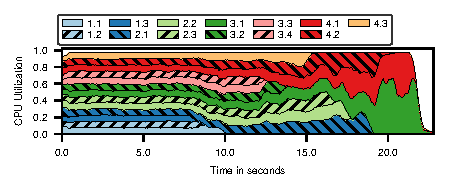
\includegraphics[width=\columnwidth]{policy/figures/ssb-all-uniform-fair-cpu-util.pdf}
	\caption{\textbf{CPU utilization of queries in fair policy}}
	\label{fig:fair-cpu-util}
\end{figure}

\subsection{Evaluation of Policies}\label{ssec:policy-eval}
In this section, we evaluate the policies that are currently implemented in the system.
%All the policies are specified in terms of the CPU resources. 
%With these experiments, 
Specifically, we verify if the actual CPU allocation among queries is in accordance with the policy specifications.
To calculate CPU utilization, we use a log of start and end times for all work orders. % and use this log to calculate the CPU utilization.

\subsubsection{Fair}
In this experiment, we execute all 13 queries from the SSB concurrently using the fair policy. 
As described in Table~\ref{table:policy-interpreatations}, the policy specification implies a fair sharing of CPU resources among concurrent queries.
The CPU utilization of the queries is depicted in Figure~\ref{fig:fair-cpu-util}.
As we can see, the CPU utilization of all the queries remains nearly equal to each other during the workload execution, despite queries belonging to different query classes with varying query complexities.

\begin{figure}[ht]
	\centering
	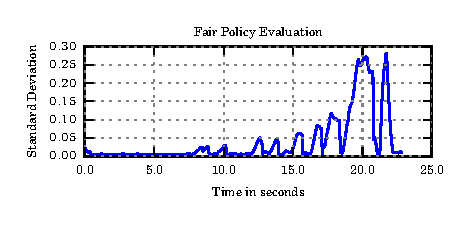
\includegraphics[width=\columnwidth]{policy/figures/fair-stddev}
	\caption{\textbf{Standard deviation of CPU utilization of active queries for fair policy}}
	\label{fig:stddev-active-queries-fair}
\end{figure}

Notice that the available CPU resources also get automatically distributed elastically among the active queries (e.g. at the 10 and 18 seconds marks) when a query finishes its execution. 
This elasticity behavior allows \sys{} to fully utilize the CPU resources at \textit{all} times.

In order to quantify the fairness metric, we compute the standard deviation of the relative CPU utilizations of queries.
At a given instant, we only consider the active queries and compute the standard deviation of their relative CPU utilizations. 

The result for this experiment can be found in Figure~\ref{fig:stddev-active-queries-fair}.
Notice that for the first 7 seconds when all 13 SSB queries are under execution, the standard deviation of CPU utilizations is nearly zero, which means the fair policy gives all queries nearly equal share of CPU. 
As more queries finish their execution, there is a transient phase (notice the peaks) after which the standard deviation drops to low levels. 
This experiment also reinforces the previous results quantitatively, and shows that the implementation is able to meet the policy specifications.

\begin{figure*}
	\centering
	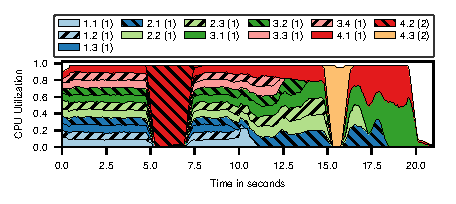
\includegraphics[width=\textwidth]{policy/figures/ssb-hpf-all.pdf}
	\caption{\textbf{CPU utilization in HPF policy. Note that $a.b  (N)$ denotes a SSB query $a.b$ with priority $N$}}
	\label{fig:hpf-all}
\end{figure*}

\subsubsection{HPF}
Now we validate if the implementation matches the 
specification of the HPF (cf. Table~\ref{table:policy-interpreatations}) policy.
%which requires that when scheduling work orders, higher priority classes be 
%preferred over lower priority classes. 

%As before, we use all the 13 SSB queries for this experiment, 
All queries have the same priority value (1) except Q4.2 and Q4.3 which have a higher priority value (2). 
The execution begins with 11 queries having the same priority value. %, i.e. Q1.1 to Q4.1.
We inject Q4.2 in the system at around 5 seconds and Q4.3 at around 15 seconds.
Figure~\ref{fig:hpf-all} shows the CPU utilization of queries during the workload 
execution.

As the high priority queries arrive (at the 5 and 15 seconds marks), the existing queries pause their execution and the scheduler makes way for the higher priority query.
As the higher priority queries finish their execution (i.e. at the 7 and 16 seconds marks), the paused queries resume their execution.

The result of this experiment also demonstrates that \sys{}'s scheduler design naturally supports query suspension, which is an important concern in workload management. 

\begin{figure*}[tp]
	\centering
	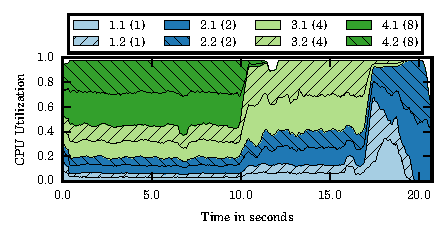
\includegraphics[width=\textwidth]{policy/figures/ssb-priority-uniform-2queries-perclass-cpu-util.pdf}
	\caption{\textbf{CPU allocation for proportional priority policy. Note that $a.b  (N)$ denotes a SSB query $a.b$ with priority $N$}}
	\label{fig:pp-cpu-util}
\end{figure*}

\subsection{Proportional Priority Policy}
Now we examine the scheduler's behavior to the proportional priority policy %(cf. Section~\ref{ssec:proportional-priority}, 
in which the higher priority integer implies higher importance.
%In this policy, the CPU allocation to query classes should be in accordance to their priority values.

We pick two queries from each SSB class, and assign them a priority value. 
Our priority assignment reflects the complexity of the queries from the corresponding class. 
For instance, query class 1 has one join, class 2 has two joins and so on.
Recall that in our implementation a higher priority integer implies higher importance.
% cf. Section~\ref{ssec:proportional-priority}.

Figure~\ref{fig:pp-cpu-util} shows the CPU allocation among concurrent queries in the proportional priority policy.
We can see that a higher priority query gets proportionally higher share of CPU as 
compared to the lower priority queries.
When all queries from the priority class 8 finish their execution (11 seconds), the 
lower priority classes elastically increase their CPU utilization, so as to use all the CPU 
resources. 
Also note that among the queries belonging to the same class, the CPU utilization is 
nearly the same, as described in the policy specifications.

\subsection{Impact of Learning on the Relative CPU Utilization}\label{ssec:learning-impact-cpu-util}

In this experiment, we compare the learning-based scheduler with a static non-learning based implementation (baseline).
We perform the comparison using fair policy, which should be the easiest policy for a static method to realize.

\begin{figure}
	\centering
	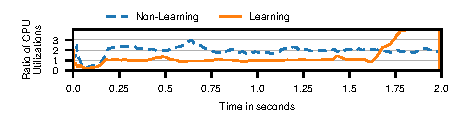
\includegraphics[width=\columnwidth]{policy/figures/q1-q11-ratio-cpu-util.pdf}
	\caption{\textbf{Ratio of CPU utilizations  $\frac{Q4.1}{Q1.1}$ for learning and non-learning 
		implementations}}
	\label{fig:non-learning-comparison}
\end{figure}

In the baseline, the probability assigned to each query remains fixed unless either a query is added or removed from the system.
If there are $N$ active concurrent queries in the system, each query gets a fixed probability $1/N$.
%In the proportional priority implementation, if the distinct priority levels are $p_1, p_2 
%\ldots p_k$, then priority $p_i$ gets a probability $\frac{p_i}{\sum\limits_{j = 
%0}^{k} 
%p_j} $.

We run $Q1.1$ and $Q4.1$ concurrently with the fair policy using both the learning and 
non-learning implementations.
Our metric for this experiment is the ratio of CPU utilizations of $Q4.1$ and $Q1.1$.
%The CPU utilization is calculated as explained in Section~\ref{ssec:policy-eval}.
As per the policy specifications, the CPU utilization for both queries in the fair policy 
should be equal. % to each other, which means the ideal ratio is 1.
Figure~\ref{fig:non-learning-comparison} shows the results of this experiment.
%We restrict the X-axis until both the queries are under execution. 

Observe in Figure~\ref{fig:non-learning-comparison}, that the ratio in the non-learning implementation is closer to 2, meaning that the 
implementation is biased towards $Q4.1$. 
This behavior stems from the fact that the time per work order for $Q4.1$ is higher than $Q1.1$ (c.f. Figure~\ref{fig:q1.1-q4.1-time-per-wo} in Appendix~\ref{apx:learning-motivation}).
In contrast, the ratio of CPU utilizations in the learning implementation is nearly 1.
The learning based implementation can identify various phases in query execution for 
both the queries and adaptively change the CPU allocation as per the changing demands 
of the queries.
The non-learning implementation however fails to recognize the fluctuations in the CPU 
demands of queries and therefore does an unfair allocation of CPU resources.
%\subsubsection{Impact of Learning on Performance}\label{sssec:makespan-comparison}
%To gauge the impact of the learning on performance, we compare the makespan (i.e. the total execution time of the entire workload) in learning vs non-learning implementations.
%For this comparison, we again use the fair policy, as earlier. 
%%in the experiment described in Section~\ref{ssec:learning-impact}.
%Table~\ref{table:makespan-learning-vs-non-learning} describes the results of the experiments using two workloads using the makespans using learning and non-learning implementations.  
%
%We can observe that the overhead of learning is negligible, in fact it benefits the makespan of the SSB workload by around 11\%, as compared to the non-learning implementation. 
%This improvement is due to a ``fairer'' allocation of CPU resources to the queries in the learning implementation.
%Longer queries don't dominate the CPU resource consumption, because of which shorter queries can finish their execution sooner.
%, thereby freeing up CPU resources available for the longer queries, which in turn can finish execution faster.
%\begin{table}
%\centering
%\begin{tabular}{|c|l|l|}
%\hline
%\multirow{2}{*}{Workload} & \multicolumn{2}{c|}{Makespan (sec)} \\ \cline{2-3} 
% & Non learning & Learning \\ \hline
%Q1.1 and Q4.1 & 4.2 & 4.3 \\ \hline
%All SSB queries & 25.6 & 22.9 \\ \hline
%\end{tabular}
%\vspace{0.5em}
%  \caption{Makespan comparison of learning and non-learning implementation}
%  \label{table:makespan-learning-vs-non-learning}
%\end{table}
%We would like to stress that the primary goal of the learning implementation is to aid the scheduler to adhere to the high level policy. 
%These experiments %described in Section~\ref{ssec:learning-impact} and Section~\ref{sssec:makespan-comparison} 
%suggest that the learning implementation not only achieves its primary goal, but also helps improving the performance of the SSB workload. 
\subsection{Impact of Learning on Performance}\label{ssec:learning-impact-perf}
Here we analyze the impact of the learning-based approach on the performance of queries. 
We use two query streams, one for $Q1.1$ and another for $Q4.1$.
%We use the same setup as the previous experiment and begin the execution with 10 queries; with five instances each of $Q4.1$ and $Q1.1$ running concurrently. 
As one instance of $Q4.1$ finishes execution, another instance of $Q4.1$ enters the system (likewise for $Q1.1$).
We compare the throughput for both $Q4.1$ and $Q1.1$ using the learning implementation of the fair policy against its non-learning implementation.

\begin{figure}[ht]
	\centering
	\begin{subfigure}[b]{0.5\textwidth}
		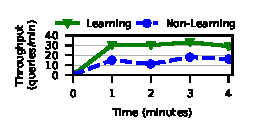
\includegraphics[width=\textwidth]{policy/figures/q11-throughput.pdf}
	\end{subfigure}%	
	~
	\begin{subfigure}[b]{0.5\textwidth}
		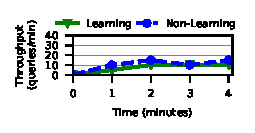
\includegraphics[width=\textwidth]{policy/figures/q41-throughput.pdf}
	\end{subfigure}%	   
	\caption{\textbf{Impact of learning on the throughput}}
	\label{fig:q11-q41-throughput}
\end{figure}

%In real life workloads, there is often a mix of queries with different query execution times.
%Based on this setting, we assume two users of the database system issuing concurrent queries. 
%One user issues short running queries and another user issues longer running queries. 
%\sys{} runs both kinds of queries concurrently using fair policy. 

%We compare the throughput observed by both users in the learning-based fair policy with non-learning based fair policy implementation, at the end of \reminder{add time} minutes from the beginning of the workload execution. 
%The concurrent query execution begins with \reminder{add number} queries, \reminder{add number} from each user.
%As soon as a user is returned the result of a query, the same user issues the next query to \sys{}, which means the think time is 0. 

%Table~\ref{table:throughput-comparison} compares the throughput observed by the two users. 
%We can observe that the throughput for the user issuing longer queries is less impacted by the change in the policy implementation. 
%However, the user issuing shorter queries is highly benefited using a learning based implementation.
%The throughput is nearly \reminder{add number}X better in the learning implementation compared to the non-learning one. 
Figure~\ref{fig:q11-q41-throughput} plots the result of this experiment and shows the throughput for each query stream. 
The throughput for the $Q4.1$ stream is not affected considerably by the choice of the implementation. 
However using the learning implementation, the throughput of the $Q1.1$ stream improves significantly (up to 3x better than the non-learning implementation). 
The reasons for the improvement are as follows:
Following the result of the previous experiment (cf. Figure~\ref{fig:non-learning-comparison}), in the non-learning implementation, $Q1.1$ which has shorter work orders, is starved of CPU resources due to $Q4.1$, which has longer duration work orders. 
In the learning-based implementation however, the $Q1.1$ stream gets its fair share of CPU resource (more than that in the non-learning implementation). 
Therefore, $Q1.1$'s performance is improved, resulting in its increased throughput. 

This experiment highlights a two-fold impact of the learning module -- first, it plays a crucial role in the fair policy enforcement. 
Second, it improves performance of queries with lower CPU requirements when they are competing with queries with higher CPU demands, thereby also increasing overall system throughput with such mixed and diverse workloads. 

\subsection{Experiment with Skewed and Uniform Data}
In this experiment we test the learning capabilities of the \sys{} scheduler under the presence and absence of skew (skew description in Section~\ref{ssec:workload}).
We execute $Q1.1$ and $Q4.1$ on the skewed and uniform data.
We sort the skewed \textit{lineorder} table on the \textit{lo\_quantity} column, to amplify the impact of skew. 
For the predicate $lo\textunderscore quantity \leq 25$ on the skewed table, some blocks have high selectivity and others have low selectivity.

%	\subfigure[$Q1.1$]{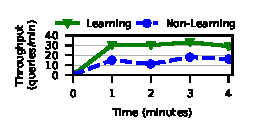
\includegraphics[width=60mm]{policy/figures/q11-throughput.pdf}}
%	\subfigure[$Q4.1$]{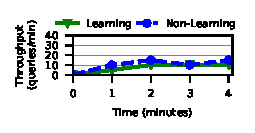
\includegraphics[width=60mm]{policy/figures/q41-throughput.pdf}}


%To test the scheduler's ability to learn in the presence of skew, 
We compare the predicted work order times for each query with its observed work order times. % for the same query.
%For completion, we perform the same experiment on the skewed data and uniform data. 
%For this experiment, we use both the skewed and uniform data.
Figure~\ref{fig:pred-vs-observed-time-per-wo} presents the results of this experiment, with relative error of the prediction on the Y-axis and time on X-axis.
We can see that the relative error is very low in both the datasets for both queries. 
The execution of $Q1.1$ with skewed data takes longer than the uniform dataset.
The intermediate peaks in the relative error correspond to phase change in the execution plan. 
Note that the scheduler learns the phase changes quickly, and adjusts its estimates after each phase change. 

\begin{figure}[t]
	\centering
    \begin{subfigure}[b]{0.4\textheight}
    	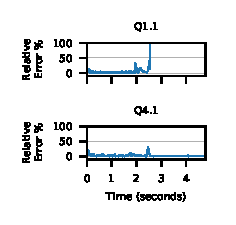
\includegraphics[width=\textwidth]{policy/figures/q11-q41-prediction-accuracy-skew-data.pdf}
	\caption{Skewed dataset}    	
    \end{subfigure}%	
	~    
    \begin{subfigure}[b]{0.4\textheight}
    	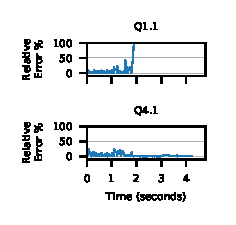
\includegraphics[width=\textwidth]{policy/figures/q11-q41-prediction-accuracy-uniform-data.pdf}
	\caption{Uniform dataset}    	    	
    \end{subfigure}%	
	\caption{\textbf{Comparison of predicted and observed time per work order}}
	\label{fig:pred-vs-observed-time-per-wo}    
\end{figure}

\subsection{Load Controller}
In this experiment, we evaluate the effectiveness of the load controller.
We use two queries from each SSB query class.
The priority value assigned to a query reflects its complexity e.g. proportional to number of joins in the query plan.
We configure the load controller with the threshold for suspending queries as 56 GB. 
As the buffer pool size grows close to the threshold, the load control mechanism kicks in.

\begin{figure}[]
	\centering
	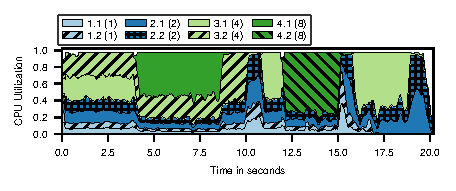
\includegraphics[width=0.6\textheight]{policy/figures/load-control-cpu-util.pdf}
	\caption{\textbf{Load control: An SSB query $a.b$ with priority $N$ is denoted as $a.b (N)$}}
	\label{fig:load-control-cpu-util}
\end{figure}

%Recall from Section~\ref{sec:background} that the 
\sys{}'s buffer pool stores the relational tables as well as hash tables used for joins and aggregations.
%The LRU-k based buffer pool implementation may evict cold pages if there is a need to make more memory available.
If the requested memory cannot be allocated, the load controller can suspend a query with the highest memory footprint. 
In the current implementation, we check for reactivating the suspended query upon every query completion. % using similar memory considerations as those described above. 
Figure~\ref{fig:load-control-cpu-util} shows the CPU utilization of the queries.

The execution begins with 6 queries.
At around 4 seconds, a higher priority query $Q4.1$ enters the system.
At this point $Q3.1$ has the highest memory footprint and the load controller
picks it as the victim for suspension.
We can observe in Figure~\ref{fig:load-control-cpu-util}, that from 4 to 11 seconds, the CPU utilization of $Q3.1$ is zero, reflecting its suspended state.
The same pattern is repeated as another high priority $Q4.2$ enters the system at around 12 seconds.
Once again $Q3.1$, that has the highest memory footprint, is suspended in order to allow $Q4.2$ to enter the system. 
Observe that in the 12 to 15 seconds time interval, $Q4.2$ gets executed and the suspended query $Q3.1$ doesn't utilize any CPU resource.

This experiment demonstrates the load control capabilities of the \sys{}
scheduler. 
It stresses an important feature of our scheduler, which integrates load-controller functionality. %closely with the resource allocation components, 
Thus, admission control and query suspension is handled holistically by the scheduler. 
